%%
% Please see https://bitbucket.org/rivanvx/beamer/wiki/Home for obtaining beamer.
%%
\documentclass{beamer}

\usetheme{Luebeck}
\usecolortheme{crane}
\setbeamertemplate{section in toc}[ball unnumbered]
\setbeamertemplate{subsection in toc}[ball unnumbered]

\usepackage[T1]{fontenc}
\usepackage{beramono}
\usepackage{graphicx}
\usepackage{hyperref}
\usepackage{pifont}
\usepackage{listings}
\usepackage{xcolor}
\usepackage{multicol}


%\definecolor{darkgreen}{rgb}{0.,0.6,0.}

\newcounter{questionizeIndex}

\newenvironment{questionize}[1][0]{%
    \setbeamercovered{invisible}%
    \setcounter{questionizeIndex}{#1}%
    \begin{itemize}%
}{ %
    \end{itemize}%
}

\newcommand{\question}[2]{%
    % #1: question
    % #2: answer (replaces question)
    \stepcounter{questionizeIndex}%
    \item<\value{questionizeIndex}->%
    \only<\value{questionizeIndex}>{#1}%
    \stepcounter{questionizeIndex}%
    \only<\value{questionizeIndex}->{#2}%
}

\newcommand{\lquestion}[4]{%
    % #1: question label
    % #2: question
    % #3: answer label
    % #4: answer (replaces question)
    \stepcounter{questionizeIndex}%
    \item[\only<\value{questionizeIndex}->{\alt<\value{questionizeIndex}>{#1}{#3}}]<\value{questionizeIndex}->%
    \only<\value{questionizeIndex}>{#2}%
    \stepcounter{questionizeIndex}%
    \only<\value{questionizeIndex}->{#4}%
}

\newcommand{\cquestion}[2]{\question{#2}{\color{#1}{#2}}}

\newcommand{\ctrue}[1]{\cquestion{darkgreen}{#1}}
\newcommand{\cfalse}[1]{\cquestion{red}{#1}}

\newcommand{\ltrue}[1]{\lquestion{\textbf{?}}{#1}{$\checkmark$}{#1}}
\newcommand{\lfalse}[1]{\lquestion{\textbf{?}}{#1}{$\times$}{#1}}

\lstset{
    basicstyle=\footnotesize\ttfamily,
    breaklines=true
}


\hypersetup{%
  colorlinks=true,% hyperlinks will be black
  pdfborderstyle={/S/U/W 1}% border style will be underline of width 1pt
}
\begin{document}

\title{MSiA414 SEC01\\ Text Analytics}
\subtitle{Lab 6 - NER}
\author{Timo Wang}
\institute{Northwestern University}
\date{October 19th, 2021}

\begin{frame}
    \titlepage
\end{frame}

%\begin{frame}{Overview}
%    \tableofcontents[hideallsubsections]
%\end{frame}

\section{What is NER tagging?}
\begin{frame}
    \frametitle{What is NER?}
    NER stands for \textbf{n}amed \textbf{e}ntity \textbf{r}ecognition. It is a method for extracting relevant entities from a large corpus and assigning them with a predefined category.
\end{frame}

\begin{frame}
    \frametitle{What is NER?}
    \begin{figure}
        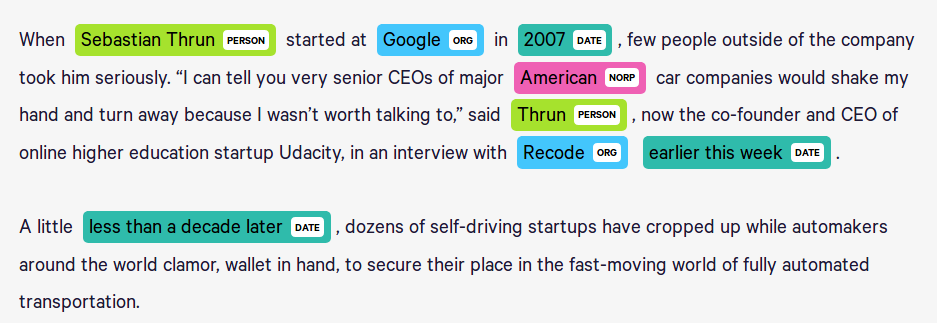
\includegraphics[scale=0.3]{ner_example}
        \caption{In this example, there are four different categories.}
    \end{figure}
\end{frame}


\section{What makes NER tagging difficult?}
\begin{frame}
    \frametitle{What makes NER tagging difficult?}
    \begin{figure}
        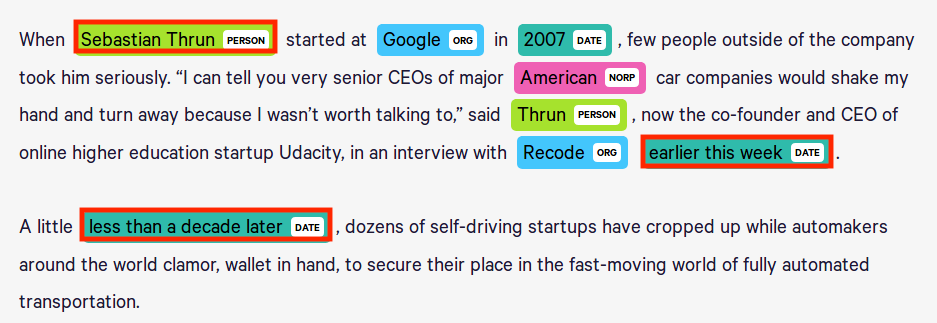
\includegraphics[scale=0.3]{ner_example_difficult}
        \caption{Notice that some entities comprise actually more than one word. We need explicitly the context information to determine the correct tag for a word.}
    \end{figure}
\end{frame}

\section{Conditional random fields (CRF)}
\begin{frame}
    \frametitle{Conditional Random Field (CRF)}
    For an input sequence $\mathbf{X}$, the probability of the output vector $\mathbf{y}$ is
    \begin{equation}
        p(\mathbf{y}\, |\, \mathbf{X})
    \end{equation}
    For a binary classification problem, we can reduce it to the following and through gradient decent update the parameters used in the linear transformation.
    \begin{equation}
        p(\mathbf{y}\, |\, \mathbf{X}) = \sigma(\mathrm{T}(\mathbf{X}))
    \end{equation}
\end{frame}

\begin{frame}
    \frametitle{Conditional Random Field (CRF)}
    However, since we want to utilize certain features, especially the context words, to make predictions, we need some model that let us explicitly specify that. 
    \begin{equation}
        p(\mathbf{y}\, |\, \mathbf{X}) = \frac{1}{\mathrm{Z}(\mathbf{X})} \exp\Big(\sum^n_{i=1}\sum_j \lambda_j\mathrm{f}_j(\mathbf{X}, i, \mathbf{y}_{i-1})\Big)
    \end{equation}
    \begin{equation}
        \mathrm{Z}(\mathbf{X}) = \sum_{\mathbf{y} \in \mathbf{Y}}\sum^n_{i=1}\sum_j \lambda_j\mathrm{f}_j(\mathbf{X}, i, \mathbf{y}_{i-1})
    \end{equation}
\end{frame}

\begin{frame}
    \frametitle{Conditional Random Field (CRF)}
    $\mathrm{f}_j(\mathbf{X}, i, \mathbf{y}_{i-1}, \mathbf{y}_i)$ is a feature function which takes as input the set of input vectors $\mathbf{X}$, position of the data point we want to predict $i$, as well as the label of the data point at index $i - 1$ $\mathbf{y}_{i-1}$ .
    
    \vspace{10pt}    
    $\lambda_j$ is the weight for the $j$-th feature function and is learned through training (gradient descent).
\end{frame}

\section{What about ``automatic'' features?}
\begin{frame}
    \frametitle{What about ``automatic'' features?}
    One way to use CRF is to select our own sets of features. However, this requires very well planned feature engineering. 
    \begin{block}{Question}
        How do we avoid feature engineering? 
    \end{block}
\end{frame}

\begin{frame}
    \frametitle{What about ``automatic'' features?}
    We rely solely on the data itself and deep neural networks to uncover those features for us. 
    
    \vspace{10pt}
    
    This is essentially what bi-LSTM + CRF is based on.
\end{frame}

\begin{frame}
    \frametitle{What about ``automatic'' features?}
    \begin{figure}
        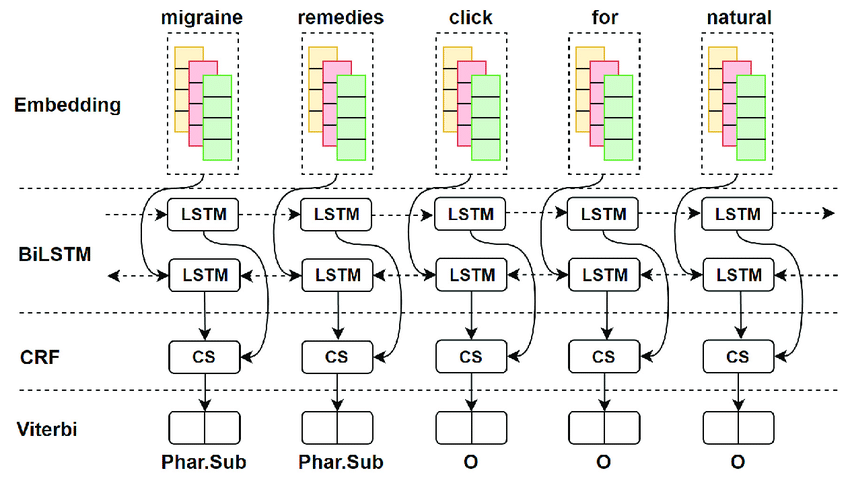
\includegraphics[scale=0.25]{bilstm-crf}
        \caption{Notice here that the CRF layer takes as input the output from the LSTM states in both directions. The values in the output vectors serve as features here.}
    \end{figure}

\end{frame}

%\section{Quiz}
%\subsection{Task 1}
%\begin{frame}
%    \frametitle{Quiz}
%    \framesubtitle{Task 1}
%\end{frame}
%
%\subsection{Task 2}
%\begin{frame}
%    \frametitle{Quiz}
%    \framesubtitle{Task 2}
%\end{frame}
%
%\subsection{Task 3}
%\begin{frame}
%    \frametitle{Quiz}
%    \framesubtitle{Task 3}
%\end{frame}

\end{document}
